\documentclass[10pt]{article}
\usepackage[margin=0.68in]{geometry}
\usepackage[T1]{fontenc}
\usepackage{graphicx}
\usepackage{array}
\setlength{\parskip}{0.42em}
\setlength{\parindent}{0pt}
\begin{document}
\begin{center}
{\Large\bfseries Full corpus ledger integrity audit}\par
{\small 2026-10-21; crypto-autoresearcher main e20013ae20d2}
\end{center}

\textbf{Method.} A full checkout held 138,890 tracked files. The repository's
\texttt{tools/validate\_ledger.py} ran with its existing prune-only baseline.
It failed on \textbf{162 unsuppressed error lines in 49 records}. It also
reported 1,210 grandfathered legacy errors and 543 advisories. None of these
counts is a count of false mathematical or performance conclusions.

\begin{center}
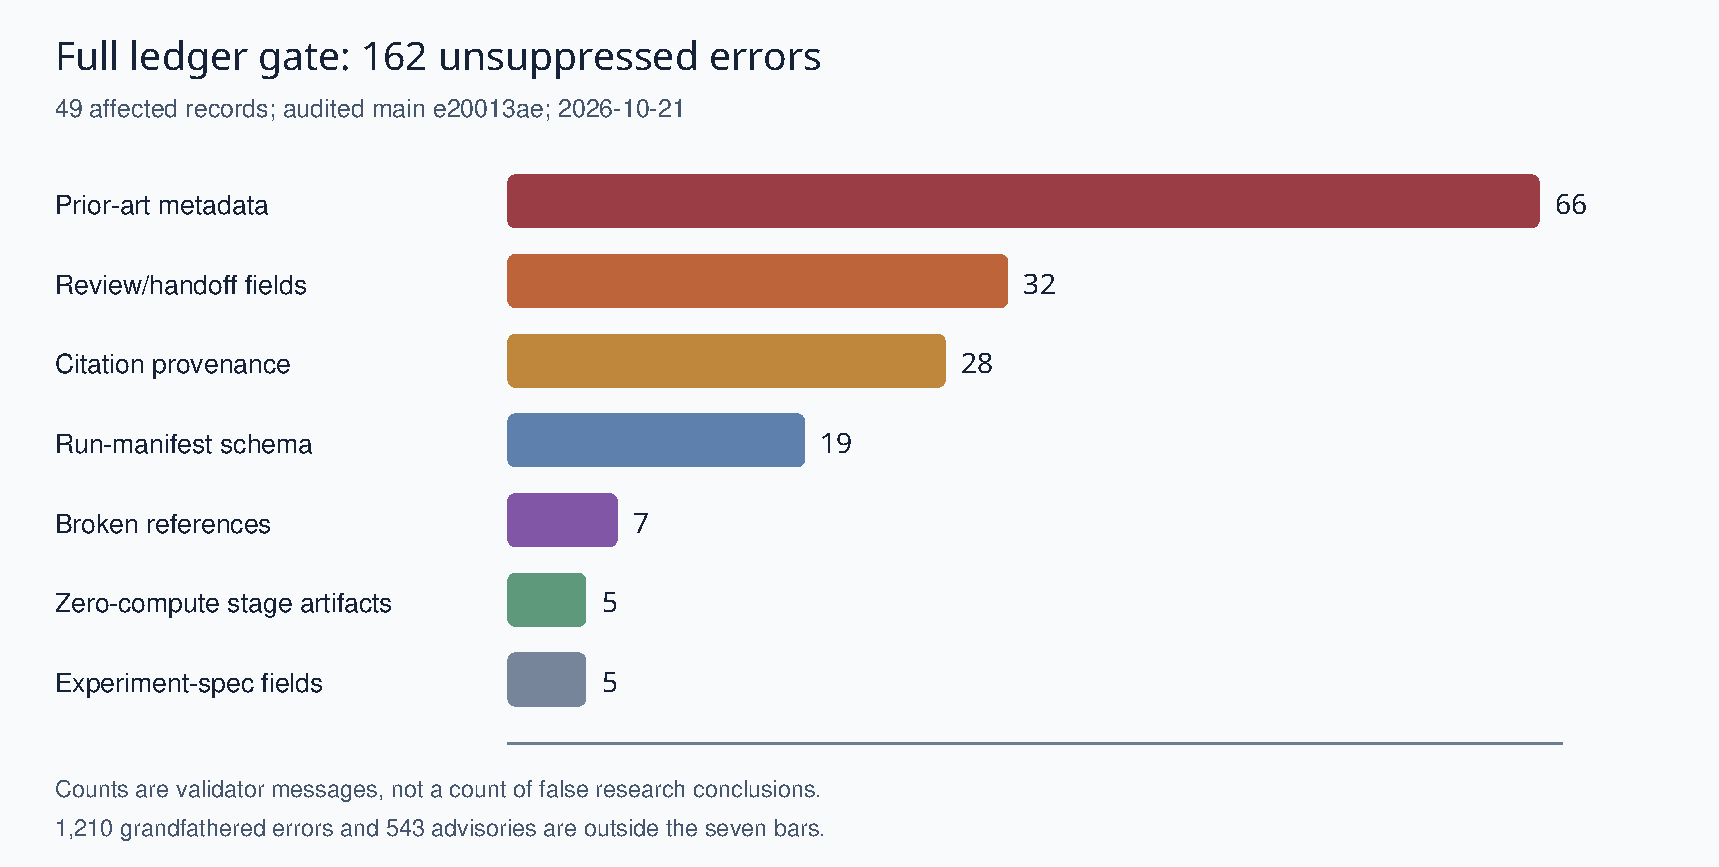
\includegraphics[width=\linewidth]{error-categories.pdf}
\end{center}

\textbf{Consequence.} The current ledger gate is red. The highest-volume
classes concern prior-art metadata, citation provenance and blind review
plans. Run-manifest and experiment-spec defects and broken references need
record-by-record repair. Five absent companion artifacts belong to a declared
zero-compute hand-derivation stage: its manifest says no program ran, so
creating synthetic stdout or raw-result files would fabricate an execution.
The classification or validator contract needs an honest repair.

\textbf{Dashboard check.} The complete-tree reader suite passed 145 tests.
The local static build emitted 55,218 files (520.6 MB); its comparison
payload carried all nine primary archived rows without a benchmark error.
A direct check of 54 fields against the current unchanged primary archive
found zero mismatches. The reader reports 24 unparseable historical source
files: nine have hash-verified, parseable supersessions and fifteen have no
registered replacement. The public Pages workflow is manually disabled; its live snapshot
still names an October 11 commit. This build is local, not a deployment or a
performance replay. The separate progress dashboard has no claim JSON inputs
and therefore no computed frontiers.

\textbf{Reader follow-on.} Nine hash-matched schema copies appear separately;
15 malformed originals are explicitly raw-only. All 24 retain their original
path, exact raw text, parse error and integrity warning. The merged reader
suite passed 146 tests. Its complete local build at b5b0b52b7c emitted
55,248 files (520.9 MB) and 27,550 records, while preserving all nine primary
benchmark rows. The current full ledger gate has the same 162 error lines in
49 paths; two new handoff advisories make 545 non-failing advisories. Hash
matching is not semantic review, and the public site has not been refreshed.
Node v22.23.3 passed a syntax check of the reader's app.js. Browser
interaction was not exercised because no browser runtime was available.

\textbf{Boundary.} The four newly supplied Lean targets and the complete
66-target machine gate are separate evidence. They do not clear these ledger
errors, independent semantic review, or historical performance validation.
No numerical graph changed because this audit produced no new timing datum.
The exact validator log, classification script, source commit and follow-up
conditions are in the accompanying Markdown report.

\end{document}
